%%%%%%%%%%%%%%%%%%%%%%%%%%%%%%%%%%%%%%%%%%%%%%%%%%%%%%%%%%%%%%%%%%%%%%%%%%%%%
%% Descr:       Vorlage für Berichte der DHBW-Karlsruhe, Ein Kapitel
%% Author:      Prof. Dr. Jürgen Vollmer, vollmer@dhbw-karlsruhe.de
%% $Id: kapitel2.tex,v 1.5 2017/10/06 14:02:51 vollmer Exp $
%%  -*- coding: utf-8 -*-
%%%%%%%%%%%%%%%%%%%%%%%%%%%%%%%%%%%%%%%%%%%%%%%%%%%%%%%%%%%%%%%%%%%%%%%%%%%

\chapter{Grundlagen}
\section{Smart Mirros \& Ambient Intelligence}
Ein smarter Spiegel ist ein interaktives System, das die Funktionalitäten eines alltäglichen Spiegels mit digitalen Anzeigen und Sensoren vereint.\footcitecustomenglisch[1]{m.v.vijayasaradhiSurveyIOTbasedSmart2022}
Ein Smart Mirror setzt sich aus einem Spionspiegel zusammen, der mit einem Display sowie einem integrierten Mikrocontroller ausgestattet ist.\footcitecustomenglisch[11]{biancoSmartMirrorEmotion2021}

% \includegraphics{}[width=\textwidth]{Images/SmartMirror.png}
\section{Raspberry Pi / Embedded Systems}
\section{Kontaktlose Pulsmessung (rPPG)}
\section{Emotionserkennung}
\section{Hardwarekomponenten}
\subsection{Industriekamera}
Industriekameras sind speziell für den Dauerbetrieb in industriellen Umgebungen ausgelegte Kamerasysteme, die sich durch robuste Mechanik, hohe Bildqualität und eine lange Lebensdauer auszeichnen.\footcitecustomlink{o.aIndustrialCameraso.J.}
Typische Einsatzgebiete von Industriekameras sind die Qualitätskontrolle in Produktionsprozessen, die Robotik sowie die Überwachung und Steuerung von Fertigungsanlagen.\footcitecustomenglisch[1-3]{javaidExploringImpactFeatures2022} Im Rahmen von Industrie 4.0 kommt ihnen eine zentrale Bedeutung zu, da sie visuelle Daten für automatisierte Entscheidungsprozesse bereitstellen.\footcitecustomebenda[1-3]{javaidExploringImpactFeatures2022}

Eine Industriekamera besteht aus mehreren zentralen Komponenten, die gemeinsam die Bildaufnahme und -verarbeitung ermmöglichen. Dazu gehören:\footcitecustomlink{zotero-item-46}
\begin{itemize}
    \item Die Linse
    \item Der Bildsensor
    \item Die Elektronik für die Signalverarbeitung
    \item Die Schnittstellen für die Datenübertragung
\end{itemize}

\subsection*{Linse}
Die Linse vergrößert die Szene indem sie das einfallende Licht bündelt und auf den Bildensensor fokusiert. Wenn die Kanten scharf sind, gilt das bild als fokussiert, andernfalls unfokussiert. Wichtige Parameter der Linse sind der Bildwinkel, das Sichtfeld, die Objektentfernung, die Brennweite und die Blende wie in Abbildung \ref{fig:linse}.\footcitecustomlink{zotero-item-46}
\begin{figure}[H]
    \centering
    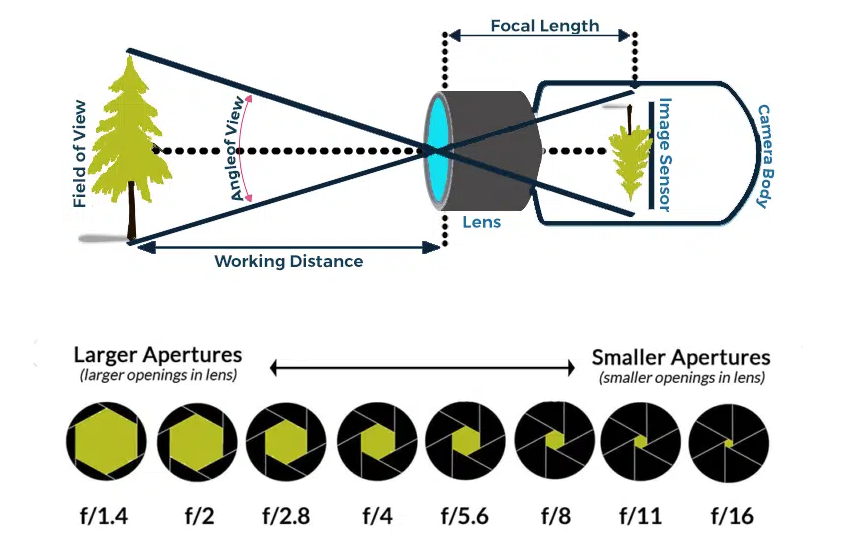
\includegraphics[width=0.5\textwidth]{Images/Lens.png}
    \caption{Schematische Darstellung einer Linse mit den wichtigsten Parametern.\protect\footnotemark}
    \label{fig:linse}
\end{figure}
\footnotetext{\found[]{zotero-item-46}}
Der Bildwinkel beschreibt den Winkel, unter dem die Kamera die Szene erfasst, während das Sichtfeld den tatsächlichen Bereich angibt, der von der Kamera abgedeckt wird. Die Objektentfernung ist die Distanz zwischen der Linse und dem fokussierten Objekt, während die Brennweite die Entfernung zwischen der Linse und dem Brennpunkt angibt. Befindet sich der brennpunkt auf dem Sensor, ist die Kamera auf das Objekt fokussiert. Die Blende steuert die Menge des einfallenden Lichts.\footcitecustomebenda{zotero-item-46}
\subsection*{Bildsensor}
\subsection{Spionspiegel}
\section{3D Druck} 